\chapter{Spiral Classification}
% Authors: Fekade Brook, Nicholas Greenquist, Aaron Wong
% Lecture date: 2/11/2019

Remember, $n$ connected linear transformations is still a linear transformation.

Let's review some of the transformations we can perform on our data. 
Linear transformations (matrices), can scale, rotate, and shear. 
In order to 'squash', we need non-linearities. 

Now, let's see how we can use PyTorch to perform classification. 

\section{Creating the Data}
% Authors: Fekade Brook, Nicholas Greenquist, Aaron Wong
% Lecture date: 2/11/2019

First, we need to import the necessary libraries:

\begin{minted}{python}
import random
import torch
from torch import nn, optim
import math
from IPython import display

from plot_lib import plot_data, plot_model, set_default
\end{minted}

Next, we need to set a constant value seed, so all random initializations are the same for all of us. 
We will also set up the dimensions of our problem. 
The entire network will map from 2D to 3D as the input layer is D, and the output layer will correspond to the number of classes, C. 
C also corresponds to the 3 possible colors we can classify each point as. 

\begin{minted}{python}
seed = 12345
random.seed(seed)
torch.manual_seed(seed)
N = 1000  # num_samples_per_class
D = 2  # dimensions
C = 3  # num_classes
H = 100  # num_hidden_units
\end{minted}

As we see above, we have H with a value of 100. 
This means we are going to map from our 2D input space to 100 dimensions. 
We do this so we can make the input easier to separate. 
We will then map it back down to 3D. 

Please note that the value of each of the 3 dimensions in the output will be the probability the point is in that class. 

Why do we even bother mapping from a low dimensional input space to higher dimensions? 
Well, it ``disentangles'' the input space so we can linearly separate it. 

Remember, we want to think of our network as having a top and a bottom. 
We want to think of the input space on the bottom and the output space at the top. 
Therefore, we want our data to be linearly separable at the top, or the end of the network. 

Before we begin training any nets on our data, we have to generate some! The code below does just that:

\begin{minted}{python}
X = torch.zeros(N * C, D)
y = torch.zeros(N * C, dtype=torch.long)
for c in range(C):
    index = 0
    t = torch.linspace(0, 1, N)
    # When c = 0 and t = 0: start of linspace
    # When c = 0 and t = 1: end of linpace
    # This inner_var is for the formula inside sin() and cos()
    # like sin(inner_var) and cos(inner_Var)
    inner_var = torch.linspace(
        # When t = 0
        (2 * math.pi / C) * (c),
        # When t = 1
        (2 * math.pi / C) * (2 + c),
        N
    ) + torch.randn(N) * 0
    
    for ix in range(N * c, N * (c + 1)):
        X[ix] = t[index] * torch.FloatTensor((
            math.sin(inner_var[index]), math.cos(inner_var[index])
        ))
        y[ix] = c
        index += 1

print("Shapes:")
print("X:", tuple(X.size()))
print("y:", tuple(y.size()))
\end{minted}

Let's view this data: 

\begin{center}
	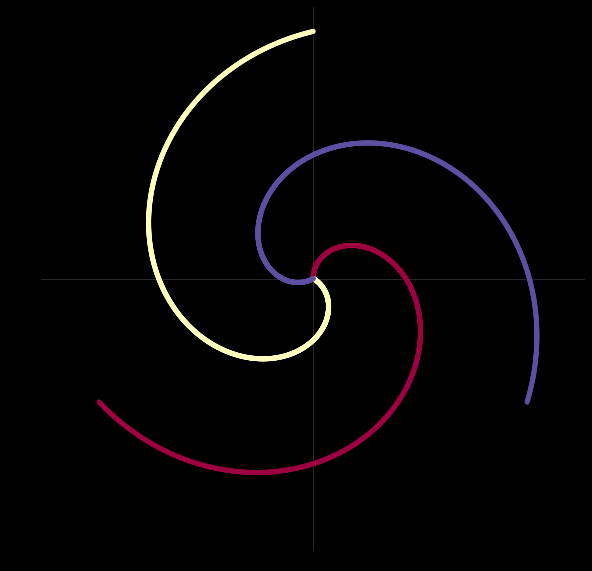
\includegraphics[width=0.5\linewidth]{lectures/03-a/images/data_no_noise.png}
\end{center}

Note that this line:

\begin{minted}{python}
torch.randn(N) * 0
\end{minted}

determines how much noise we could add to the data. 
If we change the value of 0 to be let's say .33, we get this plot: 

\begin{center}
	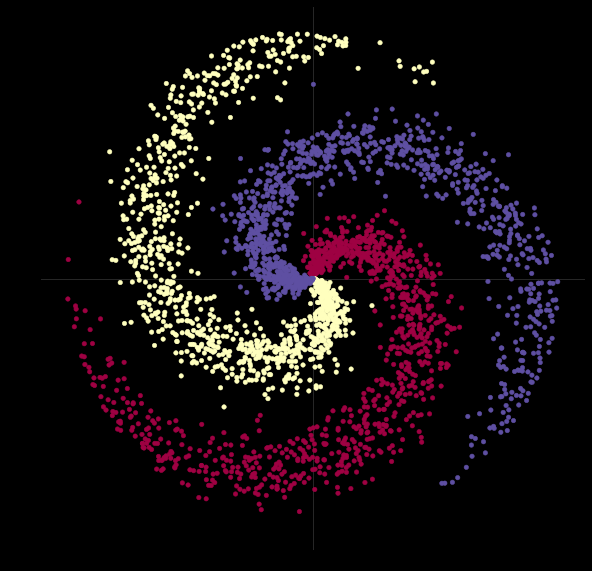
\includegraphics[width=0.5\linewidth]{lectures/03-a/images/data_noise.png} 
\end{center}


\section{Linear Model}
% Authors: Fekade Brook, Nicholas Greenquist, Aaron Wong
% Lecture date: 2/11/2019

Now, let's create a simple neural network with only linear layers.

\begin{minted}{python}
learning_rate = 1e-3
lambda_l2 = 1e-5

device = torch.device("cuda:0" if torch.cuda.is_available() else "cpu")

# nn package to create our linear model
# each Linear module has a weight and bias
model = nn.Sequential(
    nn.Linear(D, H),
    nn.Linear(H, C)
)
model.to(device) #Convert to CUDA

# nn package also has different loss functions.
# we use cross entropy loss for our classification task
criterion = torch.nn.CrossEntropyLoss()

# we use the optim package to apply
# stochastic gradient descent for our parameter updates
# built-in L2
optimizer = torch.optim.SGD(model.parameters(), lr=learning_rate, weight_decay=lambda_l2)

# Training
for t in range(1000):
    
    # Feed forward to get the logits
    y_pred = model(X)
    
    # Compute the loss and accuracy
    loss = criterion(y_pred, y)
    score, predicted = torch.max(y_pred, 1)
    acc = (y == predicted).sum().float() / len(y)
    print("[EPOCH]: %i, [LOSS]: %.6f, [ACCURACY]: %.3f" % (t, loss.item(), acc))
    display.clear_output(wait=True)
    
    # zero the gradients before running
    # the backward pass.
    optimizer.zero_grad()
    
    # Backward pass to compute the gradient
    # of loss w.r.t our learnable params. 
    loss.backward()
    
    # Update params
    optimizer.step()
\end{minted}

First, we set up some hyper parameters and then move the model to the GPU's memory if PyToch detects a GPU. 
This model will move our data from D dimensions to H dimensions, and then back to C. 

As you can see, this model uses CrossEntropyLoss to judge the performance of the classifier. 
It also uses SGD as the optimizer. 
Remember, we prefer stochastic gradient descent over batch gradient descent because most data has a lot of redundancy and we do not need to use every data point to compute the gradient. 

\textbf{epoch}: One full pass through the entire training data. 
We will sweep over every training example here 1000 times. 
That is, we will be running 1000 epochs.

Why do we have to zero the gradients before the backward pass? 
PyTorch automatically accumulates the gradients as it goes through the network. 
If we don't zero out the gradients, we keep adding new gradients to dirty memory which we don't want. 
We want to create a fresh new gradient before each step. 

Why do we add gradients to begin with? 
If we keep adding gradients, we end up with the average gradient over all the training data which is what we would end up with anyways with batch gradient descent.

\textbf{NB}: Always remember to zero your gradients! This is easily forgotten. 

What happens if we invert these two lines ? 

\begin{minted}{python}
optimizer.zero_grad()
loss.backward()
\end{minted}

We'd get nothing as the gradient would always be zero so our model would take no steps. 

What is optimizer.step()? 
This line uses the gradient to find the best direction to change the parameter weights. 
It finds the best direction and takes a ``step'' in that direction to values that give better loss. 

After running this model, we get the following decision boundaries, visualized here:

\begin{center}
	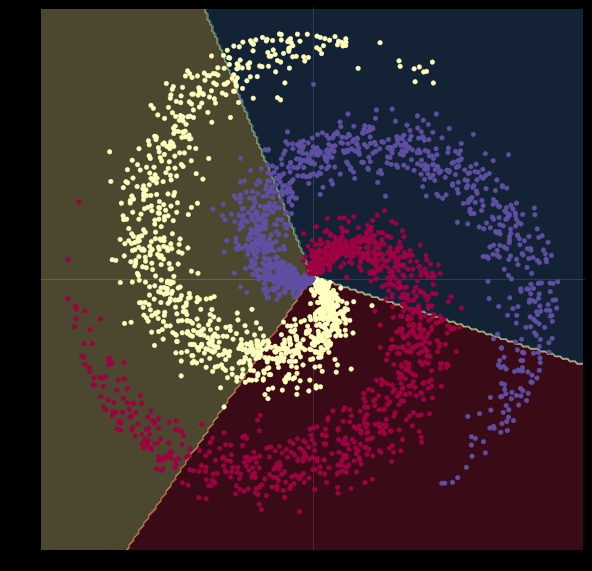
\includegraphics[width=0.5\linewidth]{lectures/03-a/images/linear.png}
\end{center}

What's wrong with this model? 
It's only giving about 50\% accuracy!

Remember, with 3 classes, random guessing would give us 33.33\% accuracy so we are still doing somewhat better than chance. 
This is because the model can do some work by simply rotating the decision boundaries. 

\textbf{NB}: Always print the initial loss before any optimizer steps. 
This is because we need to see if our model is actually improving at all from a random initialization of weights. 

Here is how to compute the initial loss for the model we have above. With three classes, we can compute what our initial loss would be by using
\begin{minted}{python}
-math.log(1/3) # 1/3 because of random guess for 3 classes
# or you can equivalently use:
math.log(3) # outputs 1.09861228867
\end{minted}

This value is what we would see with using a random guess for one of each classes. As we saw from running the notebook, with a Linear Model, we can achieve a final loss of 0.861541 which is lower than initial loss of 1.0986. Computing what the initial loss would have been with random guess and putting that into the loss function is very important because it allows us to see that after some training, we did in fact do 'better.'

\section{Non-Linear Model}
% Authors: Fekade Brook, Nicholas Greenquist, Aaron Wong
% Lecture date: 2/11/2019

Now, let's add a ReLu in between the two linear layers and see what we get.
\begin{minted}{python}
learning_rate = 1e-3
lambda_l2 = 1e-5

model = nn.Sequential(
    nn.Linear(D, H),
    nn.ReLU(),
    nn.Linear(H, C)
)
model.to(device)

# nn package also has different loss functions.
# we use cross entropy loss for our classification task
criterion = torch.nn.CrossEntropyLoss()

# we use the optim package to apply
# ADAM for our parameter updates
# built-in L2
optimizer = torch.optim.Adam(model.parameters(), lr=learning_rate, weight_decay=lambda_l2)

# e = 1.  # plotting purpose

# Training
for t in range(1000):
    
    # Feed forward to get the logits
    y_pred = model(X)
    
    # Compute the loss and accuracy
    loss = criterion(y_pred, y)
    score, predicted = torch.max(y_pred, 1)
    acc = (y == predicted).sum().float() / len(y)
    print("[EPOCH]: %i, [LOSS]: %.6f, [ACCURACY]: %.3f" % (t, loss.item(), acc))
    display.clear_output(wait=True)
    
    # zero the gradients before running
    # the backward pass.
    optimizer.zero_grad()
    
    # Backward pass to compute the gradient
    # of loss w.r.t our learnable params. 
    loss.backward()
    
    # Update params
    optimizer.step()
\end{minted}

WOW: after running this, we get a model that classifies with 0.934 accuracy. 

How does it look? 
Very pretty as you can see for yourselves below: 

\begin{center}
	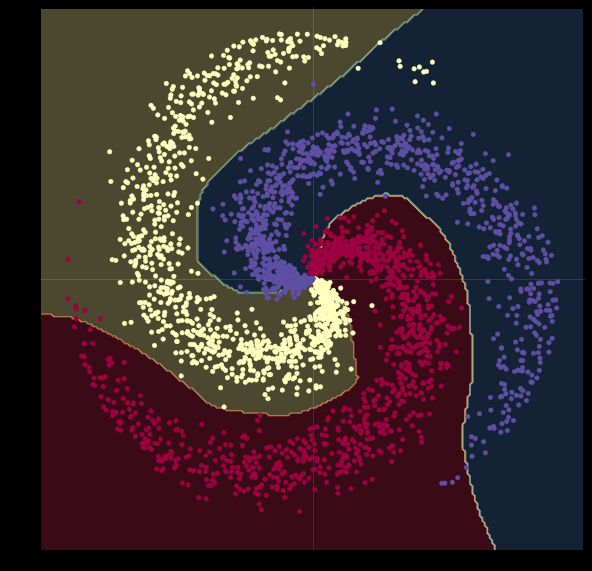
\includegraphics[width=0.5\linewidth]{lectures/03-a/images/relu.png}
\end{center}

Where are we looking from in these visualizations? 
From the bottom up! 
This is because the shape of the data we see here is before any transformations are done on it. 

\section{Skinny Model}
% Authors: Fekade Brook, Nicholas Greenquist, Aaron Wong
% Lecture date: 2/11/2019

Now, let's remove the noise of same input data. 
Let's use a neural network that doesn't expand the input to 100 dimensions this time and see what kind of classifier we get. 

\begin{figure}
	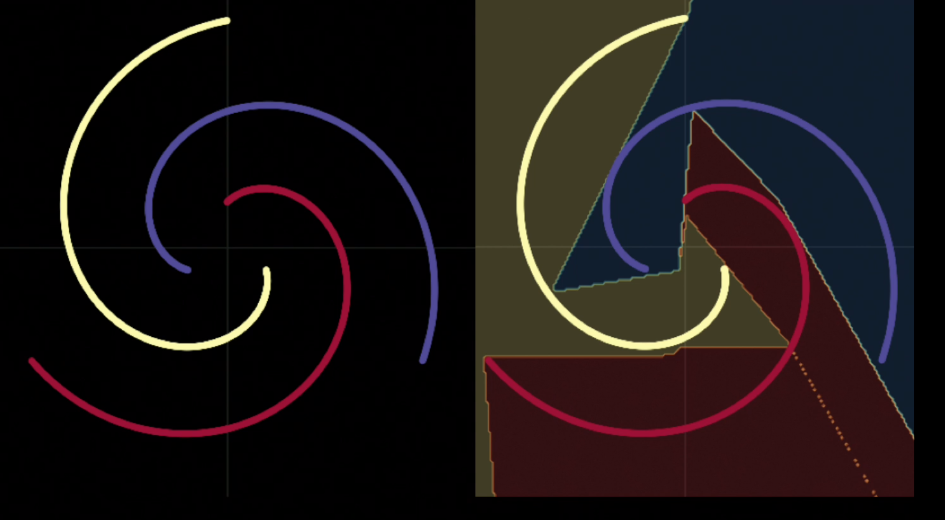
\includegraphics[width=0.85\linewidth]{lectures/03-a/images/not_wide.png}
	\caption{No projection to a higher dimension}
	\label{fig:ugly_low_dim}
\end{figure}

Here is the code that was used to generate a decision boundary like this:

\begin{minted}{python}
# NN model
def two_layer_network(D_in, D_out, hidden_layers, H):

    modules = list()
    in_d = D_in

    for l in range(hidden_layers):
        modules.append(nn.Linear(in_d, H))
        modules.append(nn.LeakyReLU())
        in_d = H
    modules.append(nn.Linear(H, H))  # added layer
    modules.append(nn.Linear(H, D_out))
    return nn.Sequential(*modules)

learning_rate = 1e-2
lambda_l2 = 1e-9

# D = 2, C = 3
model = two_layer_network(D, C, 4, D)
 
# ...use the same code as seen above to train this model
\end{minted}

The final decision boundary is very ugly and rigid. 
This is because we did not expand the dimensions of the data. 
This limits how much we can stretch out the plane to then divide the data. 
However, with enough tweaking of the random seed and rerunning the model, even this constrained model can achieve 100\% accuracy on this data as seen from \cref{fig:ugly_low_dim}. 

Let's see the entire dimension space transformed by this network:

\begin{center}
	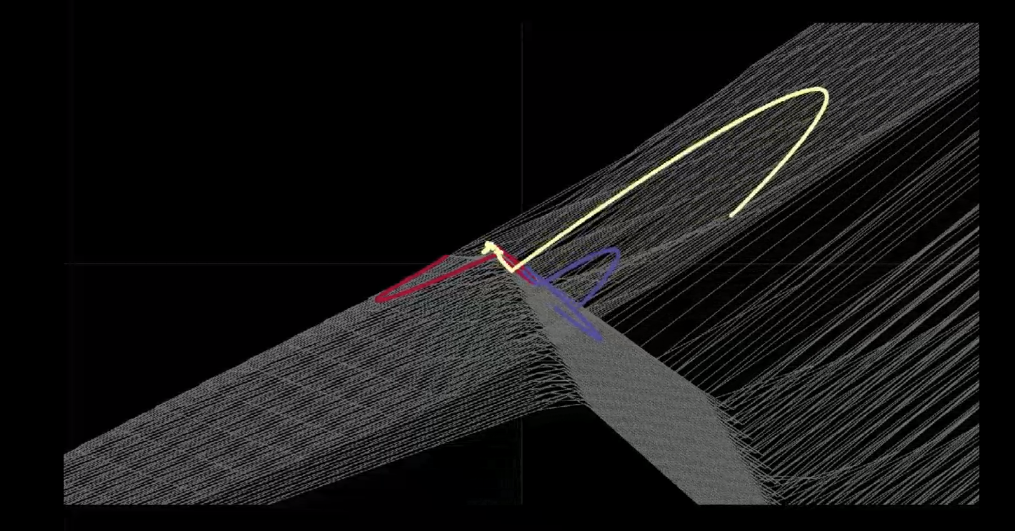
\includegraphics[width=0.85\linewidth]{lectures/03-a/images/stretch.png}
\end{center}

The network actually warps the entire space to make the spirals linearly separable. 

Now, we have seen the decision boundary from the bottom of the network. 
Let's see what the decision boundary looks like from the top of the network:

\begin{center}
	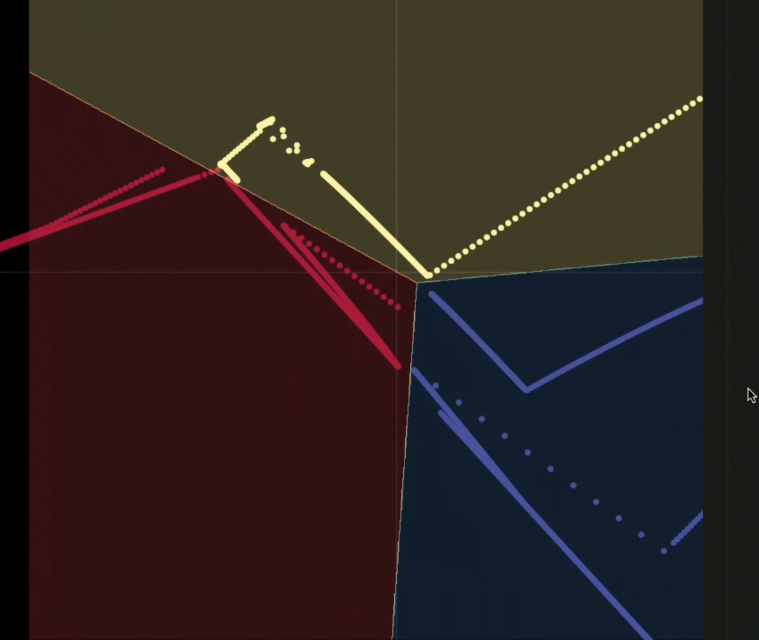
\includegraphics[width=0.5\linewidth]{lectures/03-a/images/top_view_boundary.png}
\end{center}

If you visualize the space after each transformation, you can actually see the ReLu 'cut off' negative points and 'squash' them to 0. 
Here is an example of some of the points 'squashed' by the ReLu after one step:

\begin{center}
	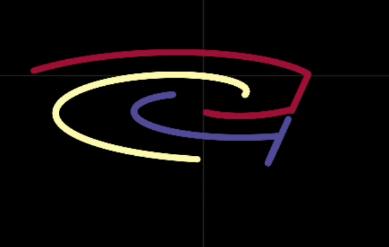
\includegraphics[width=0.85\linewidth]{lectures/03-a/images/squash.png}
\end{center}

In short, the network's job is simply to warp space until we attach a final layer that does a simple classification on the new, easily separated space. 

\noindent\fbox{\begin{minipage}{\textwidth}
\textbf{How do you know this sequence will make this space linearly separable?}
\vspace{1em}

You visually see that the space can be separated by some line. 
They aren't even overlapped so it should be easy given some specific stretching.
\end{minipage}}

One thing to notice is that if you do map to a higher dimension and then back down to the output, you will see smoother decision boundaries. 
The decision boundary we saw with this non-expansive model is more piece-wise.

If you use $\tanh$ or sigmoid non-linearities, the transitions from each new transformed dimension space are much smoother than if you clip and 'squash' with ReLu. 

As Professor LeCun stated, we get these transformations because we are letting the optimizer decide what the next best transformation to run is that minimizes the loss. 

\noindent\fbox{\begin{minipage}{\textwidth}
\textbf{What is bottom up vs top down when discussing networks? }
\vspace{1em}

Input is bottom, output is top (because you climb up hierarchy). 
If you draw the network upside down, it makes an inverted representation.
So, when we say we add classifier on top, it means we add it to the last layer in the network. 
\end{minipage}}

\noindent\fbox{\begin{minipage}{\textwidth}
\textbf{How does ReLu divide the input into subspaces?}
\vspace{1em}

This splitting actually applies to any non-linearity. 
Any time you have one in the activation function, you're basically performing elementary detection. 
So, imagine a threshold function. 
You're basically dividing the input into what section outputs the 1 and what section outputs the -1. 
However, simple threshold functions destroy too much information so we look for softer threshold functions. 
ReLu is an example of a softer threshold that preserves more information. 
\end{minipage}}

In addition to the ReLu, you can also use a Leaky ReLu: 
\href{https://medium.com/tinymind/a-practical-guide-to-relu-b83ca804f1f7}{A Practical Guide to ReLU}

According to Professor LeCun, small networks are good to visualize what is going on but will fail for most problems. 
This spiral problem requires very little width in the network so that's why it works. 

\textbf{NB}: The bigger the network, the easier it is to train as gradient descent has more time to optimize.

In addition to this note, the networks that expand to higher dimensions are trained much better and result in smoother decision boundaries. 
These boundaries are still piece-wise linear if you zoom in enough, but its almost impossible to see it from the output view. 